\section{Ergebnisse}

\subsection{Gegenseitige Validierung / Intra-DB Validierung}

\cite{intradbvalid}

\subsection{Patienten-DB}

\begin{figure}[H]
    \centering
    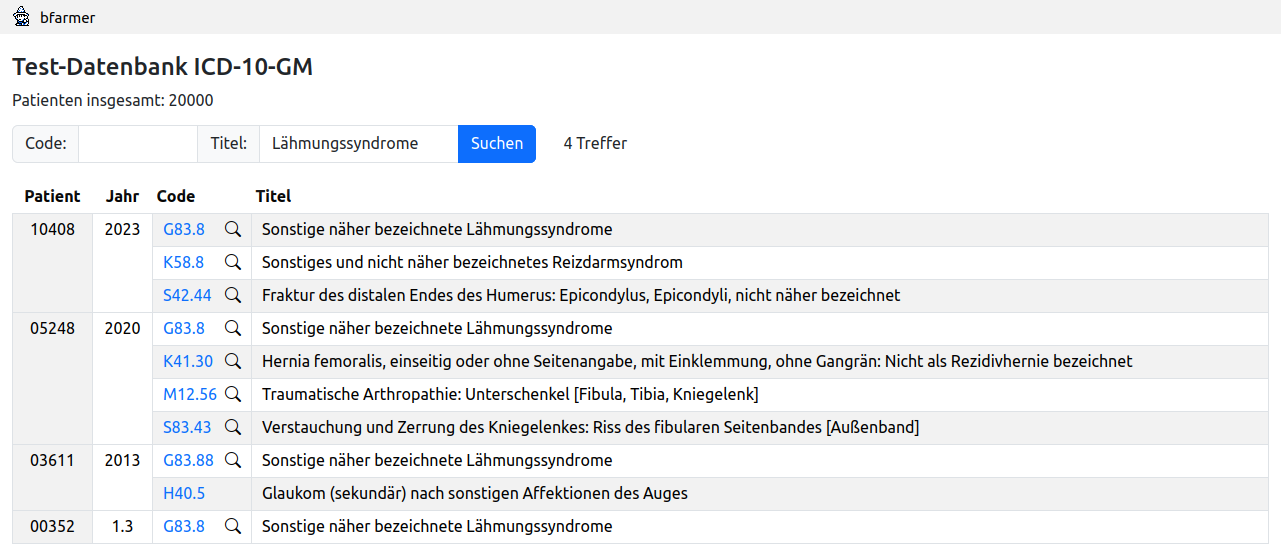
\includegraphics[width=.8\linewidth]{../img/patients_screenshot.png}
    \caption{Patienten}
\end{figure}

\begin{figure}[H]
    \centering
    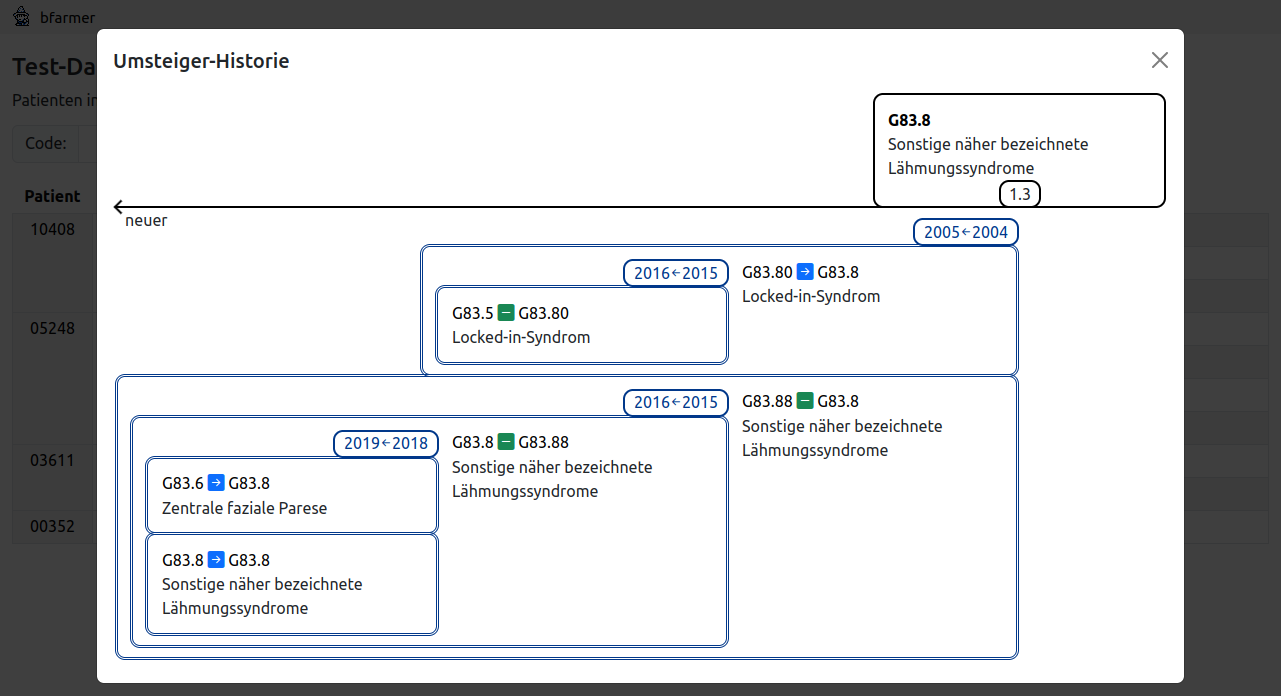
\includegraphics[width=.8\linewidth]{../img/umsteiger_screenshot.png}
    \caption{Umsteiger}
\end{figure}

Integration:

\begin{enumerate}
\item Bootstrap
\item CSS-Datei
\item On-Click Event
\item Ajax-Funktion
\end{enumerate}

\subsection{Mapping Quality}

\section{Zusammenfassung}

\section{Ausblick}

\subsection{RESTful (nach außen und innen / mehr AJAX)}

\subsection{ATC}

ATC \cite[ATC-Klassifikation]{bfarmatc}

PDF \cite{poppler}

\subsection{Sessions}

\subsection{Caching}

